\chapter{Ako robiť viac vecí naraz}

Predpokladám, že ťa zarazilo, prečo som ti v minulej časti pri programovaní grafického prostredia povedal, aby sa hralo proti \vb{RandomPlayer},
keď už máme oveľa lepšieho \vb{AlphaBetaPlayer}. Možno si aj skúsil \hbox{\vb{AlphaBetaPlayer}} použiť. Ak nie, urob to teraz. Čo si zistil? 
V programe sa funkcia \vb{plr.findMove()} sa volá pri spracovaní udalostí v hlavnom cykle. To ale znamená, že ak \vb{plr.findMove()} trvá dlho, žiadne iné udalosti
sa počas toho času nespracovávajú a program sa na tú dobu ``zasekne'' (nereaguje na pohyby myšou, neprekresľuje okno, nič...). 

Aby sme to opravili, bolo by treba \vb{findMove} rozdeliť na krátke kúsky a vždy v jednej iterícii hlavného cyklu zavolať len jeden kúsok, napr. takto:

\begin{lstlisting}
struct AlphaBetaPlayer {
  struct MoveValue {...}

  std::mt19937 rnd;
  bool thinking,finished;

  AlphaBetaPlayer();

  void startThinking(const Board& b);
  void step();
  Move getResult();

  float eval(const Board& b);
};
\end{lstlisting}

V programe by sme namiesto \vb{findMove} zavolali funkciu \vb{startThinking}. Tam sa nastaví \vb{thinking=true} a \vb{finished=false}. Hlavnú robotu bude robiť
funkcia \vb{step}, ktorá vždy prehľadá kúsok stromu a prípadne nastaví premennú \vb{finished}. V programe by to mohlo vyzerať takto:

\begin{lstlisting}
  while (running) {
    SDL_Event e;
    while (SDL_PollEvent(&e)) {
      switch (e.type) {
        ...  // spracovať ostatné typy udalostí

        case SDL_MOUSEBUTTONUP:
          if (bv.onMouseUp(e.button).from.legal() && bv.board.winner() == Empty) 
            plr.startThinking(bv.board); // krátke volanie, ktoré nastaví začiatok
          break;
      }
    }
    ... // render
    if (plr.thinking) {
      while (!plr.finished) {  // tu voláme step(), kým máme čas v rámi zvoleného fps
          plr.step();
          uint32_t now = SDL_GetTicks();
          if (now >lastFrame + msPerFrame) break;
      }
      if (plr.finished) {  // ak skončil, prečítame výsledok a nastavíme novú pozíciu
         Move m = plr.getResult();
         bv+=m;
      }
    }
    ... // prípadne SDL\_Delay, ak zostáva čas
  }
\end{lstlisting}

Ako urobiť \vb{step}? Pripomeniem, že vo \vb{findMove} robí hlavnú časť práce rekurzívna funkcia 

\begin{lstlisting}
MoveValue search(const Boardr& b, int hlbka, float alpha, float beta)
\end{lstlisting}

v nej sa, v najjednoduchšej verzii, robí zhruba takýto cyklus

\begin{lstlisting}
  auto ms = b.legalMoves();
  for (int i = 0; i < ms.size(); i++) {
    Board bb = b;
    bb += ms[i];
    float v = -search(bb, hlbka - 1, -beta, -alpha).val;
    if (v > res.val) {
      res.val = v;
      res.m = ms[i];
    }
    if (res.val > alpha) alpha = res.val;
    if (alpha >= beta) break;
  }
\end{lstlisting}

Počas rekurzívneho volania sa postupne vytvára veľa svetov pre rôzne volania funkcie \vb{search}. Ak chceme, aby sa dala prerušiť, nemôžeme použiť
rekurziu, ale bude treba, aby sme si svety vytvárali sami. Urobíme si typ, v ktorom sa dá zapamätať jeden svet funkcie \vb{search}: musí obsahovať
všetky jej parametre aj lokálne premenné, napr.

\begin{lstlisting}
struct State {
  Board b;
  int hlbka;
  double alpha, beta;
  MoveValue res;
  std::vector<Move> ms;
  int i;
};
\end{lstlisting}

\vb{AlphaBetaPlayer} potom bude mať \vb{vector<State>}, ktorý bude slúžiť ako zásobník a
kde bude mať uložené všetky rozpracované svety. Volanie \vb{search} sa pozrie na posledný svet: ak sú ešte ťahy, ktoré treba 
spracovať, tak vyrobí nový svet a pridá ho na koniec vektora, v opačnom prípade upraví hodnoty v predposlednom svete a posledný zmaže.

\begin{uloha}
  Naprogramuj prehľadávanie tak, ako sme tu povedali, aby sa dalo v grafickom prostredí hrať.
\end{uloha}

Keď si vyriešil predchádzajúcu úlohu, asi vidíš nevýhody tohoto prístupu. Prerobiť existujúceho hráča tak, aby vedel 
bežať ``zároveň'' so spracovaním udalostí vyžaduje veľa práce. V našom prípade bola len jedna rekurzívna funkcia,
v ktorej sa robila všetka práca, ale
keby si mal program, kde je viacero funkcií, z ktorých každá môže pracovať dlho a vzájomne sa volajú, celé by to 
bolo ešte oveľa zložitejšie. 

\indexItem{Alg}{vlákno {\em (thread)}}
V C++ sa dá dosiahnuť, aby viacero funkcií bežalo ``naraz'', pomocou tzv. {\em vlákien} ({\em  threads}). 
V štandardnej knižnici \vb{<thread>} je šablóna \vb{thread}, ktorá umožňuje spúšťať funkcie nezávisle od
hlavného programu. Pozri si tento program:

\vbox{
\begin{lstlisting}[label={l:thr.1}]
#include <iostream>
#include <thread>
using namespace std;

int result;

int collatz(int n) {
  int cnt;
  for (cnt = 0; n > 1; cnt++)
    if (n % 2 == 0) n = n / 2;
    else n = 3 * n + 1;
  return cnt;
}

void prvyDlhsi(int len) {
  for (result = 1; true; result++)
    if (collatz(result) > len) return;
}

int main() {
  int x;
  cin >> x;
  thread t(prvyDlhsi, x); @\ll1@
  cout << "Thread t pocita a program pokracuje" << endl; @\ll2@
  t.join(); @\ll3@
  cout << "Thread vypocital " << result << endl;
}

\end{lstlisting}
}

Funkcia \vb{prvyDlhsi} vyráta prvé číslo, ktorého Collatzova postupnosť 
(pozri Úlohu~\ref{uloha:collatz}) je dlhšia ako zadané číslo. Napr. pre vstup $512$
je výsledok $4484223$. 

V hlavnom programe sa na riadku~\ref{l:thr.1-1} vyrobí premenná \vb{t}, ktorá je typu \vb{thread}.
Jej konštruktor je šablóna, ktorá ako prvý parameter zoberie niečo spustiteľné (funkciu, 
funktor, lambdu\footnote{pripomeň si kapitolu~\ref{sec:lambdy}}) 
a spustí to. Ďalšie parametre konštruktora sú parametre, ktoré
sa použijú pri spustení\footnote{To, že konštruktor \vb{thread} 
môže mať vždy iný počet parametrov, nie je nejaká záhadná špeciálna výnimka.
Pomocou šablón sa dajú spraviť funkcie, ktoré nemajú
pevne daný počet parametrov, ale pri každom volaní môžu mať 
iný počet. Keďže ale ten zápis je zo začiatku trochu neprehľadný a nikde sme to príliš nepotrebovali,
tak som ti o tom nepovedal. Ak ťa to zaujíma, treba si nájsť kľúčové slovo {\em parameter pack},
napr. 
\dlink{https://en.cppreference.com/w/cpp/language/parameter_pack}
}. V našom prípade sa spustí funkcia \vb{prvyDlhsi(x)}.
Akonáhle sa zavolá konštruktor, thread začne pracovať nezávisle a program 
pokračuje ďalej. Hlavný program aj novovytovrený thread majú spoločnú pamäť, takže
to môže vyzerať takto:

\begin{tikzpicture}[
    boxnode/.style={font=\robotomono,draw, minimum width = 3cm},
    popis/.style ={,anchor=east, left=5mm of #1}
  ]
  \def\nxtnd[#1](#2)(#3)#4{%
  \node[boxnode,#1,rect={#1}{}{#1}{#1}, below = 0cm of #2] (#3)  {#4};
  }

  \node[boxnode,rect={}{}{}{}] (pamat) at (0,0) {pamäť};
  \node[boxnode,rect={black}{}{black}{black}, below = 0cm of pamat] (start) { };
  \nxtnd[black](start)(result){result}
  \nxtnd[teal](result)(x){x}
  \nxtnd[teal](x)(t){t}
  \nxtnd[orange](t)(len){len}
  \nxtnd[orange](len)(n){n}
  \nxtnd[orange](n)(cnt){cnt}
  \node[boxnode,rect={black}{}{black}{}, below = 0cm of cnt] { };

  
  \node[popis={result}] (global) {globálna};  \draw[->, shorten >= 2ex] (global) -- (result);
  \node[teal,popis={x}] (main) {svet {\robotomono main()}};  \draw[->, shorten >= 2ex] (main) -- (x);
  \node[orange,popis={len}] (len1) {svet {\robotomono prvyDlhsi(len)}};  \draw[->, shorten >= 2ex] (len1) -- (len);
  \node[orange,popis={n}] (cnt1) {svet {\robotomono collatz(result)}};  \draw[->, shorten >= 2ex] (cnt1) -- (n);

  \node[teal,boxnode,rect={}{}{}{}] (mainthr0) at (4,0) {hlavný program};

  \node[boxnode,rect={teal}{}{teal}{teal}, below = 0cm of mainthr0] (mainthr1) { \rule{0mm}{1cm}};
  \node[boxnode,rect={teal}{}{teal}{teal}, below = 0cm of mainthr1] (mainthr2) { \vb{thread t(...);}};
  \nxtnd[teal](mainthr2)(mainthr3){\vb{cout << ... }};
  \node[boxnode,rect={teal}{}{teal}{},  below = 0cm of mainthr3]{\rule{0mm}{6ex}};
  
  \node[orange,boxnode,rect={}{}{}{}] (tthr) at (8,0) {thread {\robotomono t}};
  \node[orange,boxnode] (tthr1) at ($ (mainthr2) + (4.5,0) $) {{\robotomono prvyDlhsi(x)}};
  \nxtnd[orange](tthr1)(tthr2){...\rule{0mm}{2ex}};
  \nxtnd[orange](tthr2)(tthr3){collatz(result)};
  \node[boxnode,rect={orange}{}{orange}{},  below = 0cm of tthr3]{\rule{0mm}{2ex}};

  \draw[teal,->,shorten >= 2ex] (mainthr2) -- (tthr1);

\end{tikzpicture}

V pamäti je globálna premenná \vb{result}. Spustí sa hlavný program (funkcia \vb{main}), ktorý vytvorí svoj svet s lokálnou premennou \vb{x}.
Potom sa vyrobí premenná \vb{t} a keď sa volá konštruktor \vb{thread} na riadku~\ref{l:thr.1-1}, spustí sa zároveň aj funkcia \vb{prvyDlhsi}, ktorá si v pamäti vyrobí svoj svet
a potom zavolá funkciu \vb{collatz}, ktorá si opäť urobí vlastný svet. 
Hlavný program beží ďalej a môže pristupovať k premenným \vb{result}, \vb{t} a \vb{x}, vnútro funkcie \vb{collatz} môže pristupovať k 
premenným \vb{result}, \vb{n} a \vb{cnt}.

\indexItem{Prg}{\vb{thread}, \vb{join}, \vb{yield}}
So samotnou premennou typu \vb{thread} sa toho moc robiť nedá, ale je dôležité, aby ostala v pamäti po celý čas, kým beží funkcia threadu. 
Nasledujúci program zavolá funkciu \vb{rob}, ktorá spustí thread s lambdou, čo dlho počíta. Funkcia \vb{rob} vzápätí skončí,
takže sa zavolá deštruktor premennej \vb{t}. Lenže príslušná funkcia ešte beží, a preto program skončí s chybou.

\begin{lstlisting}
void rob() {
  thread t([](){
    int j = 0;
    for (int i = 0; i < 100000; i++) j += i;
  });
}

int main() { rob(); }
\end{lstlisting}

Jedna z mála metód typu \vb{thread} je \vb{join}, ktorá slúži presne na to, aby sa takýmto situáciám vyhlo. 
Ak sa zavolá \vb{t.join()} (ako v našom programe na riadku~\ref{l:thr.1-3}), aktuálny thread bude čakať, kým thread z 
premennej \vb{t} dobehne. Potom je už bezpečné zavolať deštruktor.

Pri threadoch síce hovoríme, že bežia naraz, ale v skutočnosti ti to nikto nesľúbi. Väčšina procesorov má viac jadier\footnote{%
  Počet jadier sa dá zistiť pomocou \prg!cout << thread::hardware_concurrency() << endl;!.
}a každé môže v jednom momente bežať jeden thread. Kým je v celom systéme menej threadov ako jadier, systém sa spravidla snaží dať nový thread na samostatné jadro, takže thready naozaj bežia naraz.
Ak je threadov viac, musí na jednom jadre bežať viacero threadov. Niektoré systémy to robia tak, že ich striedajú: nejaký krátky čas beží jeden, potom sa preruší,
beží ďalší a tak dookola. Ale na niektorých systémoch (spravidla sú to malé procesory, ktoré sa používajú do rôznych zariadení) je také prepnutie veľmi drahé.
Robia preto to, že zoberú jeden thread a ten beží, kým sa dá: to znamená až kým neskončí alebo nezačne čakať, či už na čítanie vstupu, nejakú udalosť, alebo kvôli
volaniu ako \vb{SDL\_Delay}. Potom zoberú iný thread, ktorý chce bežať a spustia zase ten. 
Štandard jazyka C++ sľubuje len to, čo je pre všetky tieto systémy spoločné. Treba mať preto na pamäti, že pri programovaní threadov nemáš žiadnu záruku
okrem toho, že ak nejaké jadro nemá čo robiť, tak sa na ňom spustí aspoň jeden nejaký thread, ktorý chce práve bežať. 

Ak si si spustil prvý príklad, tak pravdepodobne sa text
z riadku~\ref{l:thr.1-2} vypísal hneď a potom sa čakalo na dobehnutie funkcie \vb{prvyDlhsi} v druhom threade pri volaní \vb{join}. Ale pokojne to mohlo
byť aj naopak: začal by pracovať thread \vb{t} a kým má čo robiť (v našom prípade až kým neskončí), tak ho systém nechá bežať a až keď skončí, dá slovo hlavnému threadu.
Existuje funkcia \vb{this\_thread::yield()}, ktorá signalizuje systému \cmd{Pozri sa, či nechce náhodou bežať nejaký iný thread, ktorý už dlho čaká. Ak áno, 
radšej ma preruš a začni vykonávať ten}. Čo presne sa ale stane po zavolaní \vb{yield()}, to tiež závisí od systému (štandard C++ to nijak neurčuje). 

Užitočná je aj funkcia \vb{this\_thread::sleep\_for}, ktorá robí podobnú vec ako \vb{SDL\_Delay}, totiž uspí aktuálny thread na daný čas. Kvôli čitateľnosti je 
ale navrhnutá tak, že parameter nie je \vb{int}, ale  \vb{chrono::duration}, takže treba použiť \vb{\#inlcude <chrono>} a potom použiť napr.

\begin{lstlisting}
this_thread::sleep_for(chrono::milliseconds(1234));
\end{lstlisting}

Videl si, ako vyrobiť thread, v ktorom beží nejaká funkcia. Určite si si to všimol, ale pripomeniem, že návratová hodnota z tej funkcie sa zahodí a nemáš sa k nej ako dostať.
Thready medzi sebou komunikujú tak, že jeden thread napíše do nejakej spoločnej\footnote{buď je to globálna premenná ako v našom príklade, alebo napr. pošleš ako parameter
funkcie threadu pointer na premennú a pod.} premennej a druhý odtiaľ prečíta. Možno ti v hlave zablikala kontrolka: ak nemám žiadnu kontrolu nad tým, kedy ktorý thread vykonáva ktorú časť 
svojho programu, nemôže spoločné čítanie a zapisovanie do zdieľanej premennej spôsobiť problémy? Môže, hneď ti to ukážem. Zober si nasledovný program

\vbox{
  \begin{column}{0.45}
\begin{lstlisting}
#include <iostream>
#include <set>
using namespace std;
set<int> s;

void dump() {
  for (int x : s) cout << x << " ";
  cout << endl;
} 

void rob() {
  for (int i = 5; i < 100; i++) {
    s.erase((i - 5) % 100);
    s.insert(i % 100);
    if (i % 10 == 0) dump();
  }
}

int main() {
  for (int i = 0; i < 5; i++) 
    s.insert(i);
  rob();
}
\end{lstlisting}
  \end{column}
  \hfill
  \begin{column}{0.45}

Máme v ňom globálnu množinu (t.j. vyvážený vyhľadávací strom, pozri kapitolu~\ref{sect:stromy}) \vb{s}, do ktorej na začiatku dáme čísla $0,\ldots,4$. Funkcia \vb{rob}
vždy najmenšie číslo z množiny vyberie a vloží tam o jedno väčšie. Berieme iba zvyšky po delení 100, aby bol prehľadnejší výpis. Funkcia \vb{dump} vypíše obsah množiny,
Výstup programu vyzerá takto:\\


\begin{outputBox}
6 7 8 9 10 
16 17 18 19 20 
26 27 28 29 30 
36 37 38 39 40 
46 47 48 49 50 
56 57 58 59 60 
66 67 68 69 70 
76 77 78 79 80 
86 87 88 89 90 
0 96 97 98 99 
\end{outputBox}
  \end{column}
}


Teraz program zmeňme tak, že \vb{rob} pobeží v samostatnom threade a bude množinu meniť stále dookola. Hlavný program, po tom, čo spustí thread, vždy chvíľu počká
a vypíše obsah množiny. Keď program spustíš viackrát, výstupy sa budú líšiť, ale môžu vyzerať napr. takto:


\begin{column}{0.6}
\begin{lstlisting}
#include <chrono>
#include <iostream>
#include <set>
#include <thread>
using namespace std;
set<int> s;

void dump() {
  for (int x : s) cout << x << " ";
  cout << endl;
}

void rob() {
  for (int i = 5; i < 1000000; i++) {
    s.erase((i - 5) % 100);
    s.insert(i % 100);
  }
}

int main() {
  for (int i = 0; i < 5; i++) s.insert(i);
  thread t(rob);
  for (int i = 0; i < 10; i++) {
    this_thread::sleep_for(chrono::milliseconds(1));
    dump();
  }
  t.join();
}
\end{lstlisting}
  \end{column}
  \hfill
  \begin{column}{0.3}
\begin{outputBox}
73 24 25 26 25 26 
17 23 24 
1 7 8 
8 14 15 
59 65 66 67 
8 14 15 
44 50 51 52 
61 67 68 69 
3 9 10 11 
26 32 33 34 
\end{outputBox}
  \end{column}

Čo sa stalo? Jeden thread práve robil \vb{insert} alebo \vb{erase} na vyhľadávacom strome, 
kým druhý thread ho začal prechádzať, aby ho vypisoval. Ale počas toho, ako vypisoval strom, mu prvý thread
ten strom pod rukami menil, takže sa vypísalo niečo, čo v žiadnom momente v strome nebolo. Dostali sme sa k problému, ktorému sa hovorí
\indexItem{Prg}{vzájomné vylúčenie, \vb{mutex}} {\em vzájomné vylúčenie} ({\em mutual exclusion}):
máme program, v ktorom beží viacero threadov, ale je v  ňom časť (v našom prípade manipulácia s množinou \vb{s}), v ktorej nikdy nesmie pracovať viac threadov naraz. Základným
prostriedkom na zabezpečenie
vzájomného vylúčenia je typ \vb{mutex}, ktorý je definovaný v \vb{<mutex>}. Premenné typu \vb{mutex} sa nedajú priraďovať ani kopírovať, majú dve základné metódy: \vb{lock()} a \vb{unlock()}.
Ako fungujú je opäť najlepšie vidno na príklade. Zoberme program s troma threadmi, z ktorých každý chce postupne trikrát vypísať riadok. \\

\vbox{
\begin{lstlisting}
#include <iostream>
#include <string>
#include <thread>
#include <vector>
using namespace std;

void zdrz() {  // dajme tomu, ze tu niečo zložité počíta
  for (int i = 0, j = 0; i < 100000; i++) j += i;
}       

void pis(const string &s) {
  for (int i = 0; i < 3; i++) {
    for (char c : s) {
      cout << c;
      zdrz(); 
    } 
    cout << endl;
    zdrz();
  } 
} 

int main() {
  vector<thread> ts;
  ts.push_back(thread(pis, "kedsomisielcezhoru"));
  ts.push_back(thread(pis, "STRETOLSOMTAMPOTVORU"));
  ts.push_back(thread(pis, "!$^!?#!~^*?$!"));
  
  for (auto &t : ts) t.join();
} 
\end{lstlisting}
}

Keď ho spustíš, môže to vyzerať napr.

\begin{outputBox}
Sk!Te$Rd^Es!TOo?Lm#Si!Os~Mi^Te*Al?Mc$Pe!Oz
Th!Vo$Or^Ru!U?

#kS!Te~Rd^E*sT?oO$Lm!Si
O!sM$iT^Ae!Ml?P#cO!eT~zV^hO*oR?rU$u
!
S
kTeRdEsToOmLiSsOiMeTlAcMePzOhToVrOuR
U
\end{outputBox}  

Thready sa nepredvídateľne striedajú v tom, kto práve vypíše znak.
Zmeňme teraz program tak, že pridáme \vb{\#include <mutex>}, vyrobíme globálnu premennú \vb{mutex m} a funkciu \vb{pis} zmeníme takto:

\vbox{
\begin{lstlisting}[label={l:thr.2}]
void pis(const string &s) {
  for (int i = 0; i < 3; i++) {
    m.lock(); @\ll1@
    for (char c : s) {
      cout << c;
      zdrz(); 
    } 
    cout << endl;
    m.unlock(); @\ll2@
    zdrz();
  } 
} 
\end{lstlisting}
}

Hlavný program sa nezmení, spustí tri thready. Prvý thread (nevieme, ktorý, ale jeden z nich to bude, nazvime ho $A$), sa dostane na riadok~\ref{l:thr.2-1} a zavolá \vb{m.lock()}. Tým sa mutex \vb{m}
``zamkne''. Ďalší thread, dajme tomu, že $B$, ktorý dorazí na riadok~\ref{l:thr.2-1}, tiež zavolá \vb{m.lock()}. 
Mutex \vb{m} je už ale zamknutý, preto systém thread $B$ preruší a zapamätá si, že $B$ čaká na mutex \vb{m}. Podobne aj tretí thread. Po čase thread $A$ dokončí vypisovanie reťazca
a príde na riadok~\ref{l:thr.2-2}, kde zavolá \vb{m.unlock()}. Mutex sa tým ``odomkne'', systém zistí, že nejaké thready na mutex \vb{m} čakali, vyberie z nich jeden, napr. $B$, mutex zamkne
a thread $B$ pustí bežať. Z pohľadu threadu $B$ sa nič nestalo: zavolal \vb{m.lock()} a pokračoval ďalej (medzitým chvíľu spal, ale to si nijak nevšimol). 

Na to, aby to celé fungovalo, musí byť \vb{unlock()} podporovaný
operačným systémom. Treba totiž, aby sa celá postupnosť \cmd{Odomkni mutex, zisti, či na ňom nejaké thready čakali, ak áno vyber jeden z nich, pusti ho bežať a zamkni mutex} vykonala
{\em atomicky}, t.j. ako keby to bola jedna inštrukcia. Inak by nejaký iný bežiaci thread 
mohol nájsť odomknutý mutex v tom krátkom čase medzi tým, keď 
už systém vybral nový thread na bežanie,  ale ešte nezamkol mutex.

Keď takto upravený program spustíš, už bude pracovať správne, vypíše sa napr.

\begin{outputBox}
!$^!?#!~^*?$!
STRETOLSOMTAMPOTVORU
kedsomisielcezhoru
kedsomisielcezhoru
STRETOLSOMTAMPOTVORU
!$^!?#!~^*?$!
kedsomisielcezhoru
STRETOLSOMTAMPOTVORU
!$^!?#!~^*?$!
\end{outputBox}

Akonáhle sa nejaký thread dostal do tej časti programu, v ktorej sa vypisuje, dokončil vypisovanie celého riadku bez prerušenia. Ostatné thready, ktoré by medzitým chceli 
vypisovať, poslušne čakali, kým na ne príde rad.

Použitie mutexu je veľmi náchylné na robenie chýb, ktoré sa veľmi zle hľadajú.
Keby napr. funkcia \vb{pis} zavolala \vb{return} predtým ako zavolá
\vb{m.unlock()}, mutex by ostal zamknutý a ostatné thready by sa nikdy
nedostali k slovu. Takisto mutex sa musí používať v správnom poradí, t.j.
nejaký thread zavolá \vb{lock()} a potom ten istý thread zavolá \vb{unlock()}.
Volať \vb{unlock()} z iného threadu, volať dvakrát za sebou \vb{lock()} z toho
istého threadu a pod. môže spôsobiť záhadné chyby, ktoré sa neprejavia pri
každom behu programu, ale iba občas. Preto sa \vb{mutex} používa zriedkakedy priamo,\indexItem{Prg}{\vb{lock\_guard}}
ale častejšie prostredníctvom \vb{lock\_guard}. Typ \vb{lock\_guard} v konštruktore 
dostane ako parameter premennú typu \vb{mutex} a ešte v konštruktore na ňu zavolá \vb{lock()}.
V deštruktore sa potom zavolá \vb{unlock()}. To znamená, že ak vyrobíš premennú typu
\vb{lock\_guard}, program za ňou je chránený príslušným mutexom, až kým sa nezavolá jej deštruktor.
Napr. funkcia \vb{pis} by sa dala napísať takto:

\vbox{
\begin{lstlisting}[label={l:thr.3}]
void pis(const string &s) {
  for (int i = 0; i < 3; i++) {
    { @\ll1@
      lock_guard guard(m);@\ll2@
      for (char c : s) {
        cout << c;
        zdrz();
      }
      cout << endl;
    }@\ll3@
    zdrz();
  }
}
\end{lstlisting}
}

Zložený príkaz na riadkoch \ref{l:thr.3-1} a \ref{l:thr.3-3} vytvára svet, v ktorom 
žije premenná \vb{guard}. Pri jej vytvorení sa na riadku \ref{l:thr.3-2} zamkne mutex \vb{m}
a v jej deštruktore na riadku~\ref{l:thr.3-3} sa odomkne. Príjemné na tom je, že ak 
niekedy v budúcnosti zmeníš program tak, že napr. niekedy počas vypisovania zavoláš \vb{return},
deštruktor \vb{guard} sa zavolá aj tak a nezanesieš si do programu ozaj nepríjemnú chybu.

Niekedy je ombedzenie, že ten istý thread, čo zavolal \vb{lock()} musí zavolať aj \vb{unlock()}
dosť nepríjemné. V novších\footnote{od štandardu C++20 vyššie, takže kompilátoru 
chceš povedať napr. \vb{-std=c++20}}  štandardoch C++ je
aj všeobecnejší mechanizmus, tzv. {\em semafór}. Používa sa podobne ako \vb{mutex}: \indexItem{Prg}{\vb{counting\_semapphore}}
pridá sa \vb{\#include <semaphore>} a vyrobí sa premenná typu \vb{counting\_semaphore}
niekde, kde ju všetky thready vidia (napr. ako globálna premenná).
Semafór\footnote{Pôvodne ho vymyslel E. W. Dijkstra a predstavoval si pri tom
také železničné návestie s ukazovateľom, ktorý sa môže posúvať hore a dolu.} je
vlastne počítadlo, ktoré sa dá atomicky zvyšovať a znižovať. V konštruktore
dostane štartovaciu hodnotu. Ak máš premennú napr. \vb{counting\_semaphore s(4)},
tak ktorýkoľvek thread môže hocikedy zavolať \vb{s.acquire()}, čím sa hodnota počítadla zníži, alebo
\vb{s.release()}, čím sa hodnota počítadla zvýši. Hodnota nikdy nebude záporná
a ak nejaký thread zavolá \vb{s.acquire()} vtedy, keď hodnota počítadla bola $0$, 
systém ho preruší a zapamätá si, kde čaká. Keď potom nejaký iný thread zavolá 
\vb{s.release()}, tak podobne ako pri mutexoch sa atomicky vyberie jeden z čakajúcich threadov
a spustí sa.

Preože semafór môže jeden thread zvýšiť a druhý znížiť, používajú sa na dohadovanie medzi threadmi:
jeden thread na semafóre zaspí (spraví \vb{acquire()} na nulovom počítadle) a čaká, kým ho druhý zobudí (zavolá \vb{release()}).

Typický príklad na komunikáciu threadov je \indexItem{Alg}{{\em producer-consumer}} tzv. {\em producer-consumer} problém. 
Dajme tomu, že chceš vyrobiť dataset, v ktorom budú tváre ľudí z obrázkov na internete.
Máš jednu funkciu, ktorá vie stiahnuť náhodný obrázok z internetu a druhú funkciu, ktorá vie zobrať obrázok a vyrezať z neho oblasť s tvárou.
Problém je, že obe tie funkcie môžu trvať rôzne dlho. Raz treba dlho čakať, kým sa podarí nejaký obrázok stiahnuť a inokedy sa obrázky
chrlia rýchlo, ale ich spracovanie trvá dlho. Vyriešime to tak, že si urobíme buffer, do ktorého bude prvá funkcia (nazvime ju \vb{producer})
ukladať obrázky a druhá funkcia (nazvime ju \vb{consumer}) z neho bude čítať. Na buffer môžeme použiť \indexItem{Prg}{\vb{deque}} napr. triedu \vb{deque} z STL; \vb{deque}
sa podobá \vb{vector}u, ale vieme efektívne pridávať a uberať z oboch koncov, t.j. máme
operácie \vb{push\_back}, \vb{push\_front}, \vb{pop\_back}, \vb{pop\_front}, \vb{front} a \vb{back},
ktoré vedia pridávať, uberať a pristupovať k prvkom na začiatku a konci poľa\footnote{Premysli si, ako by si si takú triedu mohol vyrobiť sám.}. 
Chceme, aby si \vb{producer} pracoval a keď získa obrázok, 
uloží ho na koniec buffra. Podobne \vb{consumer} si postupne číta z buffra obrázky a spracováva ich. Ak je buffer prázdny, \vb{consumer} by mal
zaspať a zobudiť sa, až keď bude mať robotu. Podobne nechceme, aby buffer príliš narástol, takže ak je v ňom viac ako $n$ obrázkov,
\vb{producer} by mal zaspať a zobudiť sa, až keď bude v buffri miesto. No a ešte by sme chceli aj takú možnosť, aby bežalo naraz viac threadov
\vb{producer} a viac threadov \vb{consumer}.

Aby sme zabezpečili, že buffer sa nikdy nepokazí, budeme si prístup k nemu chrániť mutexom \vb{mtx}. Zároveň si jednotlivé \vb{producer} a \vb{conumer}
thready budú signalizovať, kedy majú zaspať a kedy sa majú zobudiť. Na to použijeme dva semafóry. Semafór \vb{prazdny} bude mať vždy takú hodnotu
počítadla, koľko je v buffri vecí. Začína teda s nulou, \vb{consumer} ho zníži a \vb{producer} ho zvýši. Druhý semafór, \vb{plny}, bude mať hodnotu počítadla
vždy takú koľko je v buffri voľných miest. Celý systém by vyzeral takto:

\hfill
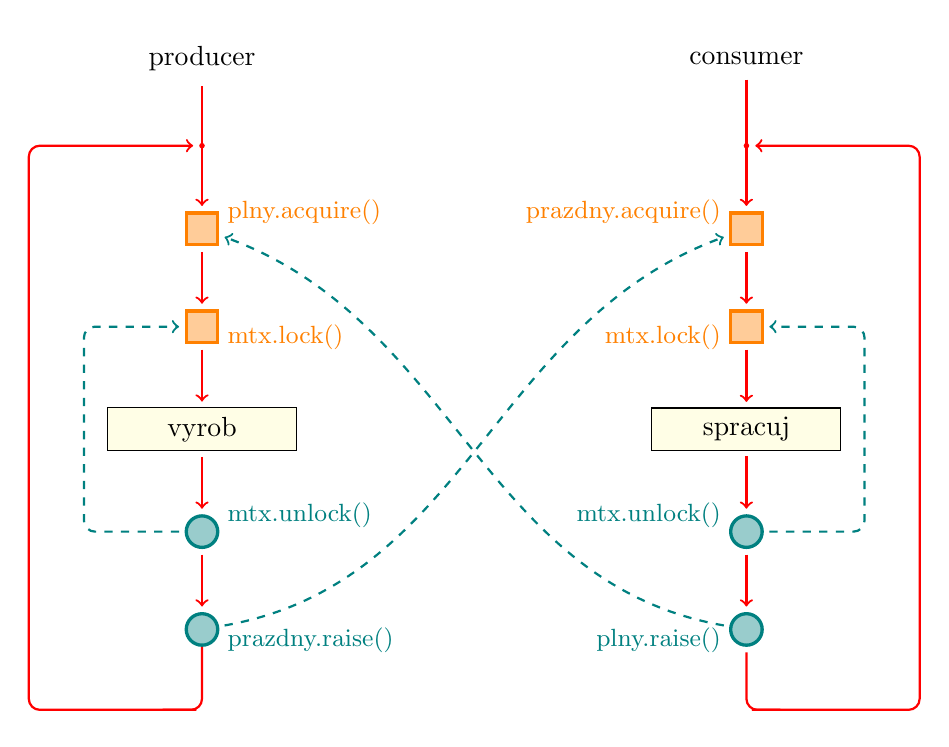
\begin{tikzpicture}[
    head/.style={font=\robotomono},
    point/.style={circle,inner sep=0pt,minimum size=2pt,fill=red},
    lock/.style={fill=orange!40!white, draw=orange, very thick, minimum size=4mm,rectangle},
    unlock/.style={fill=teal!40!white, draw=teal, very thick, minimum size=4mm,circle},
    work/.style={draw=black, thin, fill=yellow!10!white, minimum width=24mm, font=\robotomono},
    ctrl/.style={thick, shorten <= 2pt, shorten >= 2pt, rounded corners},
    skip loop/.style={->, to path={-- ++(#1,0) |- (\tikztotarget)}}
]
    \matrix[column sep = 4.5cm, row sep = 8mm]{
    \node[head] (p0) {producer}; & \node[head] (c0){consumer}; \\
    \node[point] (p1){} ; & \node[point] (c1){}; \\
    \node[lock] (p2) {}; & \node[lock] (c2){}; \\
    \node[lock] (p3) {}; & \node[lock] (c3){}; \\
    \node[work] (p4) {vyrob}; & \node[work] (c4){spracuj}; \\
    \node[unlock] (p5) {}; & \node[unlock] (c5){}; \\
    \node[unlock] (p6) {}; & \node[unlock] (c6){}; \\
    \coordinate (p7) ; & \coordinate (c7);\\
  };

  \path (p7) edge [red, ctrl, skip loop = -22mm] (p1)
        (c7) edge [red, ctrl, skip loop = 22mm] (c1);
         
  \foreach \s in {p,c} { \foreach \n/\m in {0/2,2/3,3/4,4/5,5/6} { \draw[red, ctrl, -> ] (\s\n) -- (\s\m);}}

  \draw[red, ctrl]   (p6) -- (p7) -- ++(-5mm,0)
                     (c6) -- (c7) -- ++(5mm,0);

  \path (p5) edge [dashed, teal, ctrl, skip loop = -15mm] (p3)
        (c5) edge [dashed, teal, ctrl, skip loop = 15mm] (c3);

  
  \def\lblr#1(#2)[#3]#4{\node[#3, anchor = west] at (#2) {\raisebox{#1 5mm}{\hspace*{2mm}\robotomono\small #4}}}
  \def\lbll#1(#2)[#3]#4{\node[#3, anchor = east] at (#2) {\raisebox{#1 5mm}{\robotomono\small #4\hspace*{2mm}}}}

  \lblr-(p6)[teal]{prazdny.raise()};
  \lblr+(p5)[teal]{mtx.unlock()};
  \lblr+(p2)[orange]{plny.acquire()};
  \lblr-(p3)[orange]{mtx.lock()};

  \lbll-(c6)[teal]{plny.raise()};
  \lbll+(c5)[teal]{mtx.unlock()};
  \lbll+(c2)[orange]{prazdny.acquire()};
  \lbll-(c3)[orange]{mtx.lock()};

  \path (p6) edge[teal, dashed, ctrl, ->, out=10, in=200] (c2)
        (c6) edge[teal, dashed, ctrl, ->, out=170, in=340] (p2);

\end{tikzpicture}
\hfill~

Na tento obrázok  sa treba dobre zadívať a presvedčiť sa, že je to naozaj v poriadku, nech by thready pracovali v akomkoľvek poradí: 
keď si \vb{producer} zamkne \vb{mtx}, v buffri je voľné miesto, keď si 
\vb{consumer} zamkne \vb{mtx}, je v buffri aspoň jedna vec. \indexItem{Alg}{{\em deadlock}}Zároveň nikdy nenastane {\em deadlock}, t.j. situácia, keď všetky thready spia a 
čakajú a celý program sa tým pádom zasekne.

Keď už máme program takto navrhnutý, napísať ho je ľahké. Tu urobíme iba simuláciu, namiesto vyrábania aj spracovávania dáme iba čakanie.
Najprv si pripravíme knižnice a globálne premenné. Tu si len treba všimnúť, že \vb{counting\_semaphore} je šablóna, ktorá ako parameter
dostane očakávanú maximálnu hodnotu počítadla\footnote{Ako sme už spomínali, šablóny môžu mať okrem typov aj celočíselné parametre, napr.
pre šablónu \prg!template <typename T, int N> int f(T x) {return (int)(x) + N;}! je \prg!f<float, 4>! funkcia, ktorá zoberie parameter typu \prg!float!,
pretypuje ho na \prg!int! a priráta k nemu $4$. Hodnota $4$ je v tele funkcie fixovaná, pre rôzne hodnoty sa zo šablóny vyrobia rôzne funkcie.}. Je to viac-menej iba
kvôli možnej optimalizácii, v programe môže počítadlo narásť aj viac.


\begin{lstlisting}
#include <chrono>
#include <deque>
#include <iostream>
#include <mutex>
#include <random>
#include <semaphore>
#include <thread>
#include <vector>
using namespace std;
const int N = 10;

deque<int> buffer;

counting_semaphore<N> plny(N), prazdny(0);
mutex mtx;
\end{lstlisting}

Pre jednoduchosť povieme, že \vb{producer} aj \vb{consumer} budú bežať stále. V naozajstnom programe by si tam chcel mať nejaký spôsob, ako ich zastaviť (napr. zdieľanú
premennú, do ktorej sa zapíše, ak treba skončiť). V našom prípade si \vb{producer} vymyslí číslo, chvíľu počká a uloží ho na koniec buffra.

\vbox{
\begin{lstlisting}
void producer(int id) {
  mt19937 rnd{random_device{}()};

  while (true) {
    int num = rnd() % 1000;
    this_thread::sleep_for(chrono::milliseconds(rnd() % 1000));
    plny.acquire();
    mtx.lock();
    cout << "Producer " << id << " vyrobil " << num << endl;
    buffer.push_back(num);
    mtx.unlock();
    prazdny.release();
  }
}
\end{lstlisting}
}

Podobne napíšeme \vb{consumer}:

\vbox{
\begin{lstlisting}
void consumer(int id) {
  mt19937 rnd{random_device{}()};

  while (true) {
    prazdny.acquire();
    mtx.lock();
    int num = buffer.front();
    buffer.pop_front();
    cout << "Consumer " << id << " spracoval " << num << endl;
    mtx.unlock();
    plny.release();
    this_thread::sleep_for(chrono::milliseconds(rnd() % 1000));
  }
}
\end{lstlisting}
}

Hlavný program len spustí thready:

\begin{lstlisting}
int main() {
  vector<thread> ts;
  for (int i = 1; i <= 4; i++) ts.push_back(thread(producer, i));
  for (int i = 1; i <= 2; i++) ts.push_back(thread(consumer, i));
  for (auto &t : ts) t.join();
}
\end{lstlisting}

Toto by nateraz mohlo stačiť na základný prehľad o multithreadovom programovaní. Keď sa vrátime k nášmu \btr projektu: namiesto zložitého prerábania hráča, ako na začiatku tejto 
kapitoly, je jednoduchšie zaobaliť existujúceho hráča do threadu. V konštruktore sa spustí thread, ktorý spí na semafóre. Keď treba rátať ťah, semafór sa zdvihne a thread počíta.
Hlavný program pri spracovaní udalostí kontroluje, či hráčov thread už dorátal ťah.

\begin{uloha}
  Naprogramuj multithreadového hráča.
\end{uloha}

